\documentclass[12pt,letterpaper]{report}
\usepackage[margin=1in]{geometry}
\usepackage{graphicx}
\usepackage{amsmath}
\usepackage[font=small,labelfont=bf]{caption}
\usepackage[justification=centering]{caption}
\usepackage{tikz}
\usepackage{circuitikz}
\usepackage{siunitx}
\usepackage{float}
\newlength \figwidth
\setlength \figwidth {0.75\linewidth}

\begin{document}

\title{E153 Laboratory Assignment \#5}
\author{Courtney Keeler and Stephen Pinto\\
Harvey Mudd College}
\date{October 21, 2013}
\maketitle

\section*{List of Materials}
\begin{itemize}
	\item Tektronix 2212 Oscilloscope
	\item Pomona 4550B (10X probe)
	\item Elenco LCM-1950 Multimeter
	\item 2N3904 transistor
	\item Lab Station 7 Transformer (s.n. 139 01 665)
	\item Simpson 260 (s.n. 139 01 156)
	\item Model EUW-28 Resistance Substitution Box (s. n. 77901165)
	\item 10 kOhm potentiometer
\end{itemize}

\section*{Purpose}
The purpose of this lab is to build bi-polar transistor circuits and do neat things with them.

\section*{4.1 Transistor Junctions}
\subsection*{Procedure}

\begin{enumerate}
\item Obtain a 2N3904 transistor and measure the voltage across the the BC junction using the diode test function
\item Repeat the previous step for the BE junction
\end{enumerate}

\subsection*{Results}

\begin{table}[ht]
\caption{Voltage across each "diode"} % title of Table
\centering 
    \begin{tabular}{| c | c |} 
    \hline
    $V_{\text{BC}}$ & 0.711 V \\
    $V_{\text{BE}}$ & 0.717 V \\
    \hline
    \end{tabular}
    \label{table:section_1}
\end{table}

\subsection*{Analysis}

We are looking to see if the transistor is in working condition. If it is, the two junctions BE and BC will look like back to back forward biased diodes when testing them with the digital multimeter's diode test function. As shown in Table \ref{table:section_1}, each junction has a drop of 0.7 V, just like a forward biased diode - meaning the transistor is working.

\section*{4.5 Transistor Current Gain}
\subsection*{Procedure}

\begin{enumerate}
\item Construct the circuit shown in Figure \ref{fig:4.5_circuit}
\item Start with an initial R (from the resistance substitution box) of 4.7 MOhm
\item Measure $I_C$ and $I_B$ using two digital multimeters
\item Turn on both power supplies and record the currents
\item Repeat for enough values of R to cover three decades of collector current.
\end{enumerate}

\begin{figure}[H]
\centering
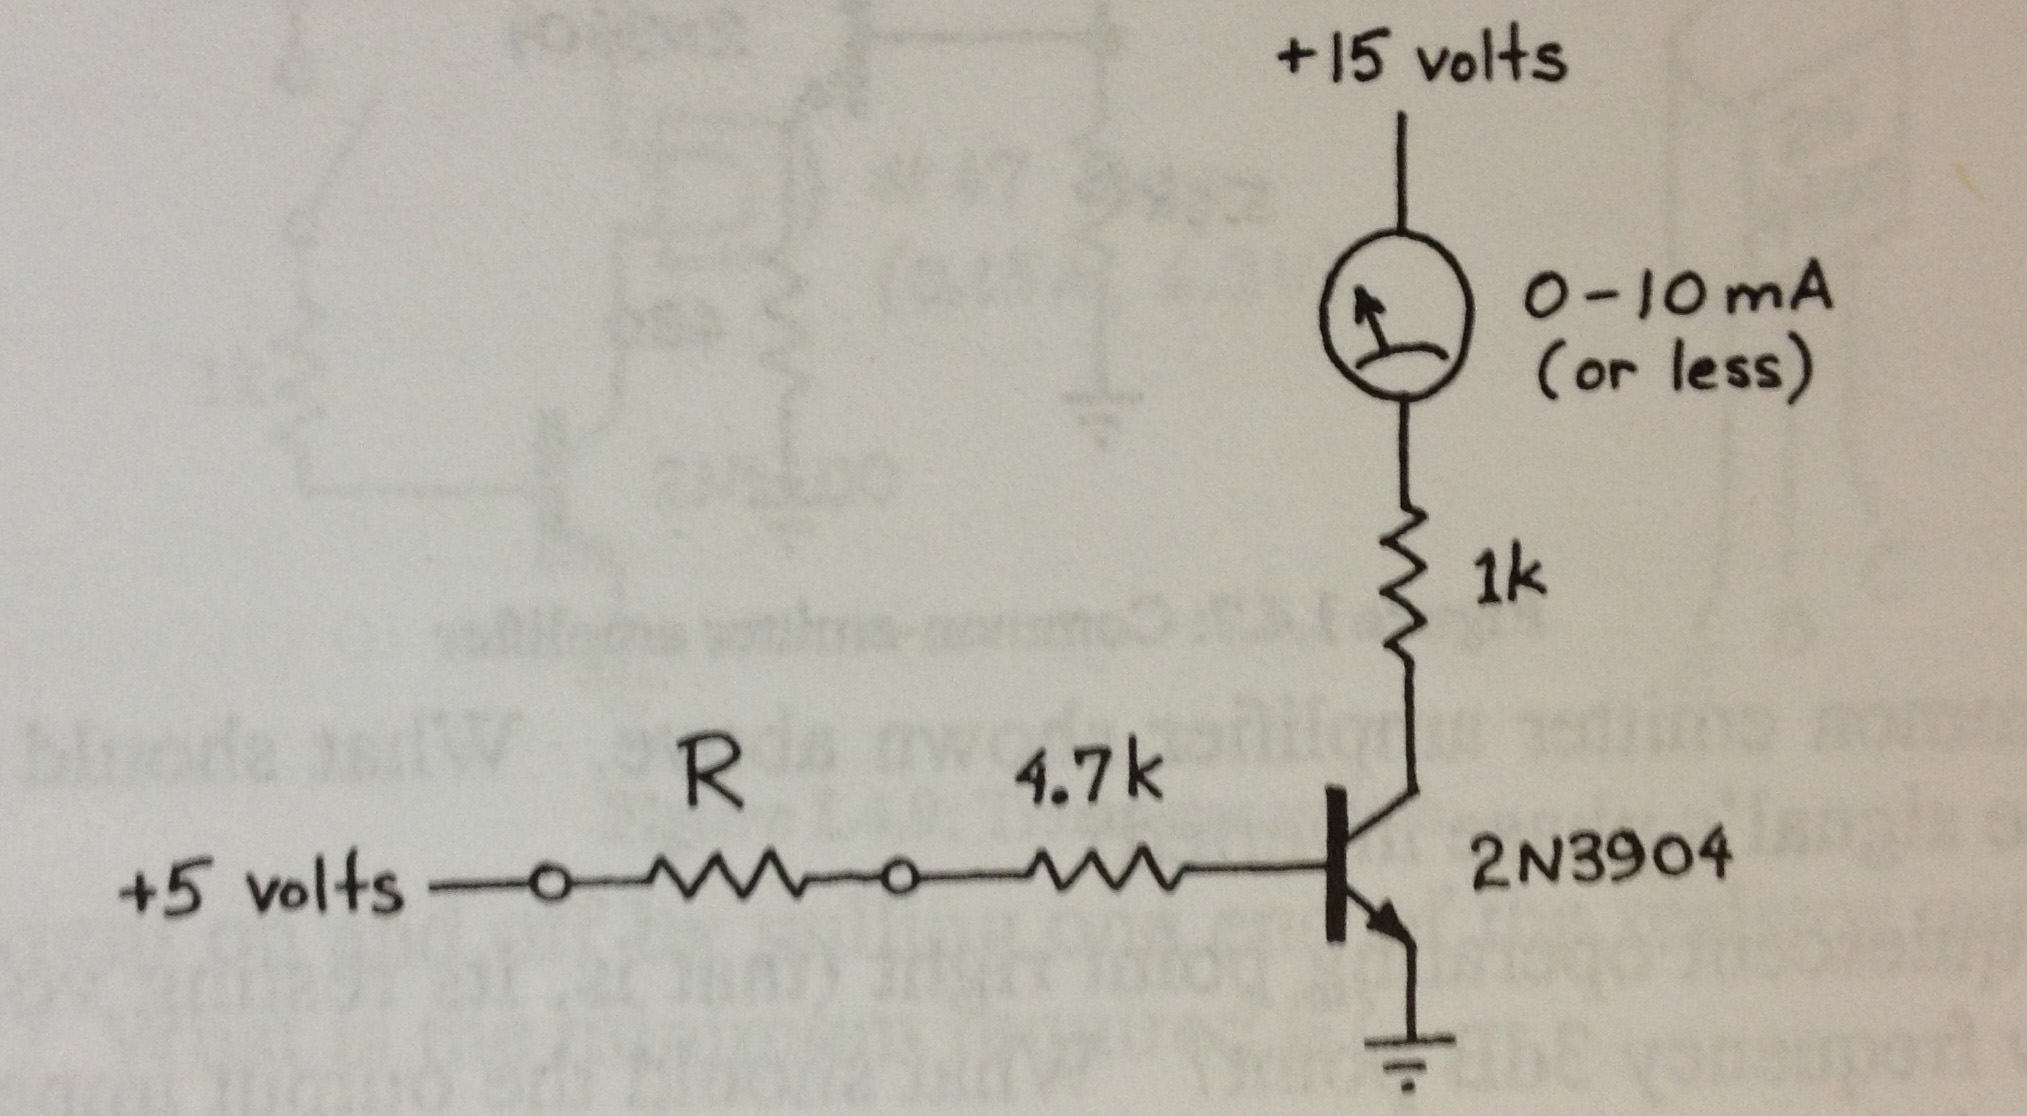
\includegraphics[width=\figwidth, keepaspectratio=true]{lab5/circuit_2.jpg}
\caption{Output waveform of the diode limiter when the input is a 2 $\text{V}_{\text{pp}}$ 8 kHz square wave.}
\label{fig:4.5_circuit}
\end{figure}

\subsection*{Results}
Note that 
$$
\beta = \frac{I_C}{I_B}
$$
and
$$
I_B = \frac{V_{R_B}}{R_B}.
$$

\begin{table}[ht]
\caption{Experimental Results for part 4.5} % title of Table
\centering 
    \begin{tabular}{| c | c | c | c | c | c |}
    \hline  
    $R$ & $R_B$ & $I_C$ & $V_{R_B}$ & $I_B$ & $\beta$\\
    \hline
    10 M$\Omega$  & 4.7 k$\Omega$ & 0.09 mA & 2.0 mV  & 0.43 uA & 212 \\
    470 k$\Omega$ & 4.7 k$\Omega$ & 1.7 mA & 39.8 mV  & 8.47 uA & 201 \\
    100 k$\Omega$ & 4.7 k$\Omega$ & 8.1 mA & 197.7 mV & 42.1 uA & 193 \\
    \hline
    \end{tabular}
    \label{table:4_5_results}
\end{table}

\section*{4.6 Current Source}
\subsection*{Procedure}

\begin{enumerate}
\item Construct the current sink circuit shown in Figure \ref{fig:4.6_circuit}
\item Slowly vary the 1 kOhm potentiometer while looking for changes in the measured collector current (use a digital ammeter).
\item Monitor the $V_{CE}$ using a digital voltmeter
\item Observe what happens at the maximum resistance of the pot
\end{enumerate}

\begin{figure}[H]
\centering
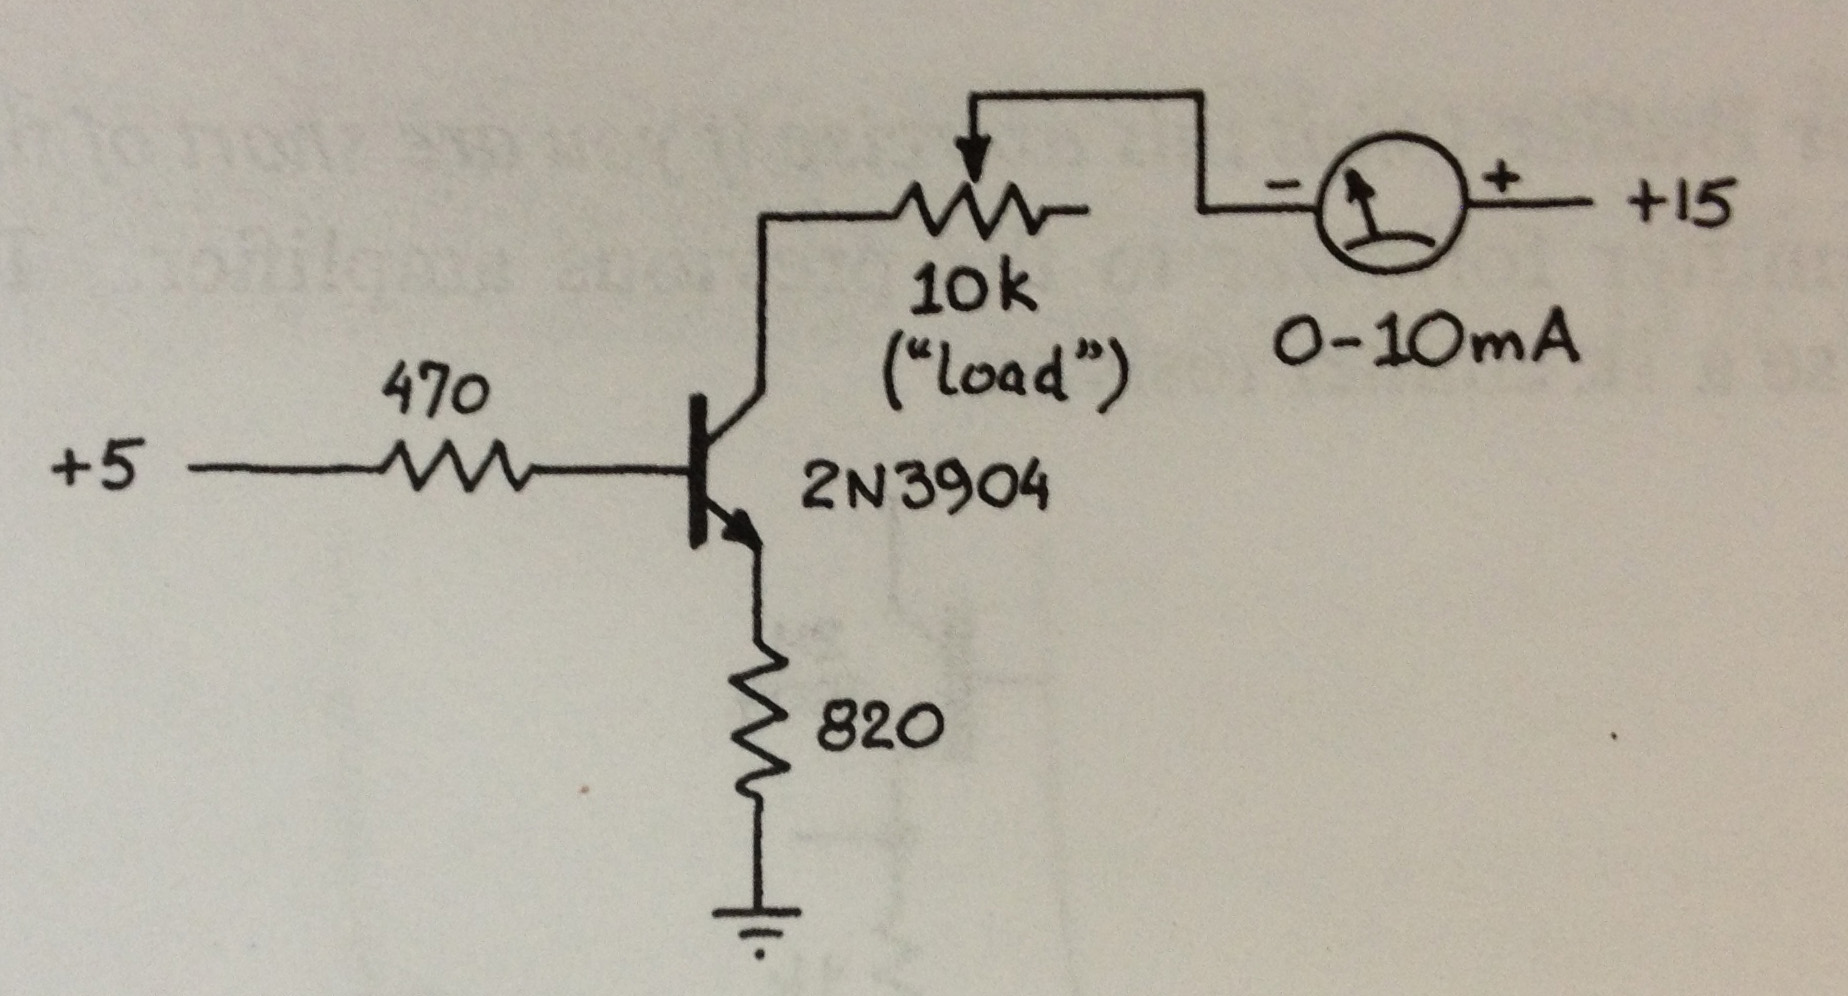
\includegraphics[width=\figwidth, keepaspectratio=true]{lab5/circuit.jpg}
\caption{Output waveform of the diode limiter when the input is a 2 $\text{V}_{\text{pp}}$ 8 kHz square wave.}
\label{fig:4.6_circuit}
\end{figure}

\subsection*{Results}
Since the slope of the transistor's $I_C$ vs. $V_{CE}$ curve is so shallow, it was difficult to accurately measure changes in $I_C$ as the potentiometer varied. The only two datapoints collected are summarized in Table \ref{table:4-6_results}

\begin{table}[ht]
\caption{Experimental Results for part 4.5} % title of Table
\centering 
    \begin{tabular}{| c | c |}
    \hline  
    $I_C$ & $V_{CE}$\\
    \hline
    5.29 mA & 2.85 V\\
    5.30 mA & 6.53 V\\
    \hline
    \end{tabular}
    \label{table:4-6_results}
\end{table}

\subsection*{Analysis}
The compliance range of this transistor is roughly 0.2 V upward (limited by the 15 V source of course.) This compliance range covers a change of about 0.02 mA in the collector current. Using the two data points in Table \ref{table:4-6_results}, the slope of the $I_C$ vs $V_{CE}$ curve is
$$
m = \frac{5.30 mA - 5.29 mA}{6.53V - 2.85V} = 2.7 \frac{\mu A}{V}
$$
Which makes the Early voltage
$$
V_A = \frac{5.29 mA}{2.7 \frac{\mu A}{V}} - 2.85 V = 1944 V
$$

Explain the max resistance behavior in terms of voltage compliance of the current source

What causes the variations in output current as the load is varied within the compliance range? Verify by explanation and by making the appropriate measurements


\end{document}
